%!TEX root = CooperBarba2014.tex

The implicit-solvent model describes the mean-field potential in a molecular system using continuum electrostatics. A system where a protein is dissolved in a solvent is defined by two dielectric regions interfaced by the solvent-excluded surface (\ses). The \ses determines the closest a water molecule can get to the protein, and we generate it by rolling a spherical probe of the size of a water molecule around the protein (Figure \ref{fig:forcefield-ses}). The dielectric constant inside the protein is low ($\epsilon= 2\text{ to }4$) and there are point charges located at the positions of the atoms. On the other hand, the solvent region has the dielectric constant of water $\epsilon \approx 80$, and we need to account for the presence of salt. This model results in a system of partial differential equations where the Poisson equation describes the electrostatic potential inside the protein, and the linearized Poisson-Boltzmann equation governs outside the protein. Appropriate interface conditions on the \ses express the continuity of the potential and electric displacement, completing the mathematical formulation.

\begin{figure}% [h]
   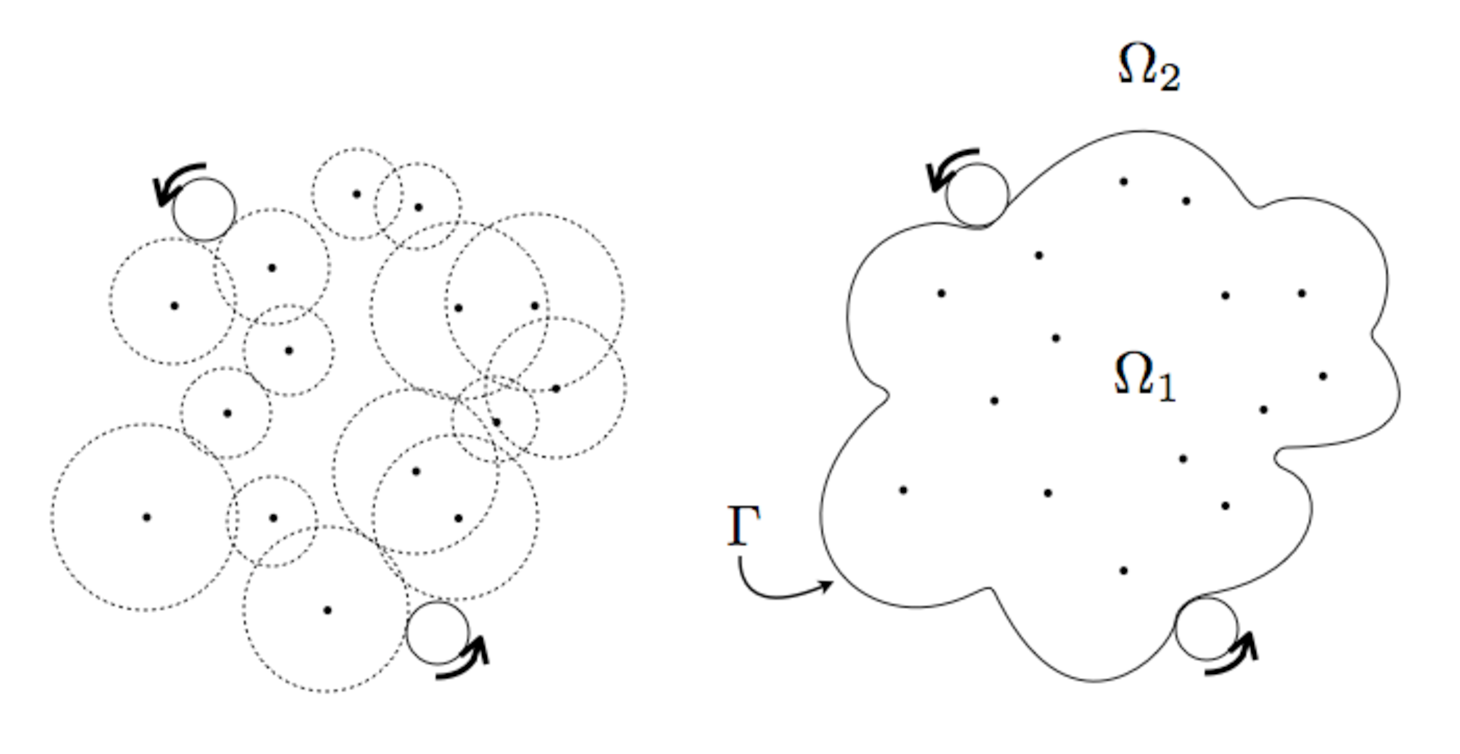
\includegraphics[width=0.49\textwidth]{Figure1.pdf} 
   \caption{Sketch of the process for generating a solvent-excluded surface (\ses): a protein molecule contains a set of atoms that define a radius upon applying a force field and a probe the size of a water molecule is rolled to define the  \ses. $\Omega_1$ is the protein region and $\Omega_2$ the solvent region.}
   \label{fig:forcefield-ses}
\end{figure}

In this work, we use an extension of the implicit-solvent model to consider the effect of charged surfaces. Such is the case of the setup sketched by Figure \ref{fig:molecule_surface}, which is described mathematically by the following equations:


\begin{align} \label{eq:pde}
\nabla^2 \phi_1(\mathbf{r}) &= - \sum_k \frac{q_k}{\epsilon_1} \delta(\mathbf{r},\mathbf{r}_k) \ \text{ in solute $(\Omega_1)$,}  \nonumber \\ 
\nabla^2\phi_2 (\mathbf{r}) &= \kappa^2 \phi_2(\mathbf{r}) \quad \qquad \ \ \ \text{ in solvent $(\Omega_2)$,}  \nonumber \\ 
\phi_1 &=\phi_2 \nonumber \\ 
\epsilon_1 \frac{\partial \phi_1}{\partial \mathbf{n}} &= \epsilon_2 \frac{\partial \phi_2}{\partial \mathbf{n}}  \ \qquad \qquad \text{ on interface $\Gamma_1$, and} \nonumber \\
-\epsilon_2 \frac{\partial \phi_2}{\partial \mathbf{n}} &= \sigma_0 \qquad \qquad \qquad \text{ on surface $\Gamma_2$} 
\end{align}

\noindent Here, $\phi_i$ is the potential corresponding to the region $\Omega_i$ with permittivity $\epsilon_i$, and $\sigma_0$ is the set charge on the nanosurface. The surface $\Gamma_2$ could correspond to a device such as a biosensor.

\begin{figure}
   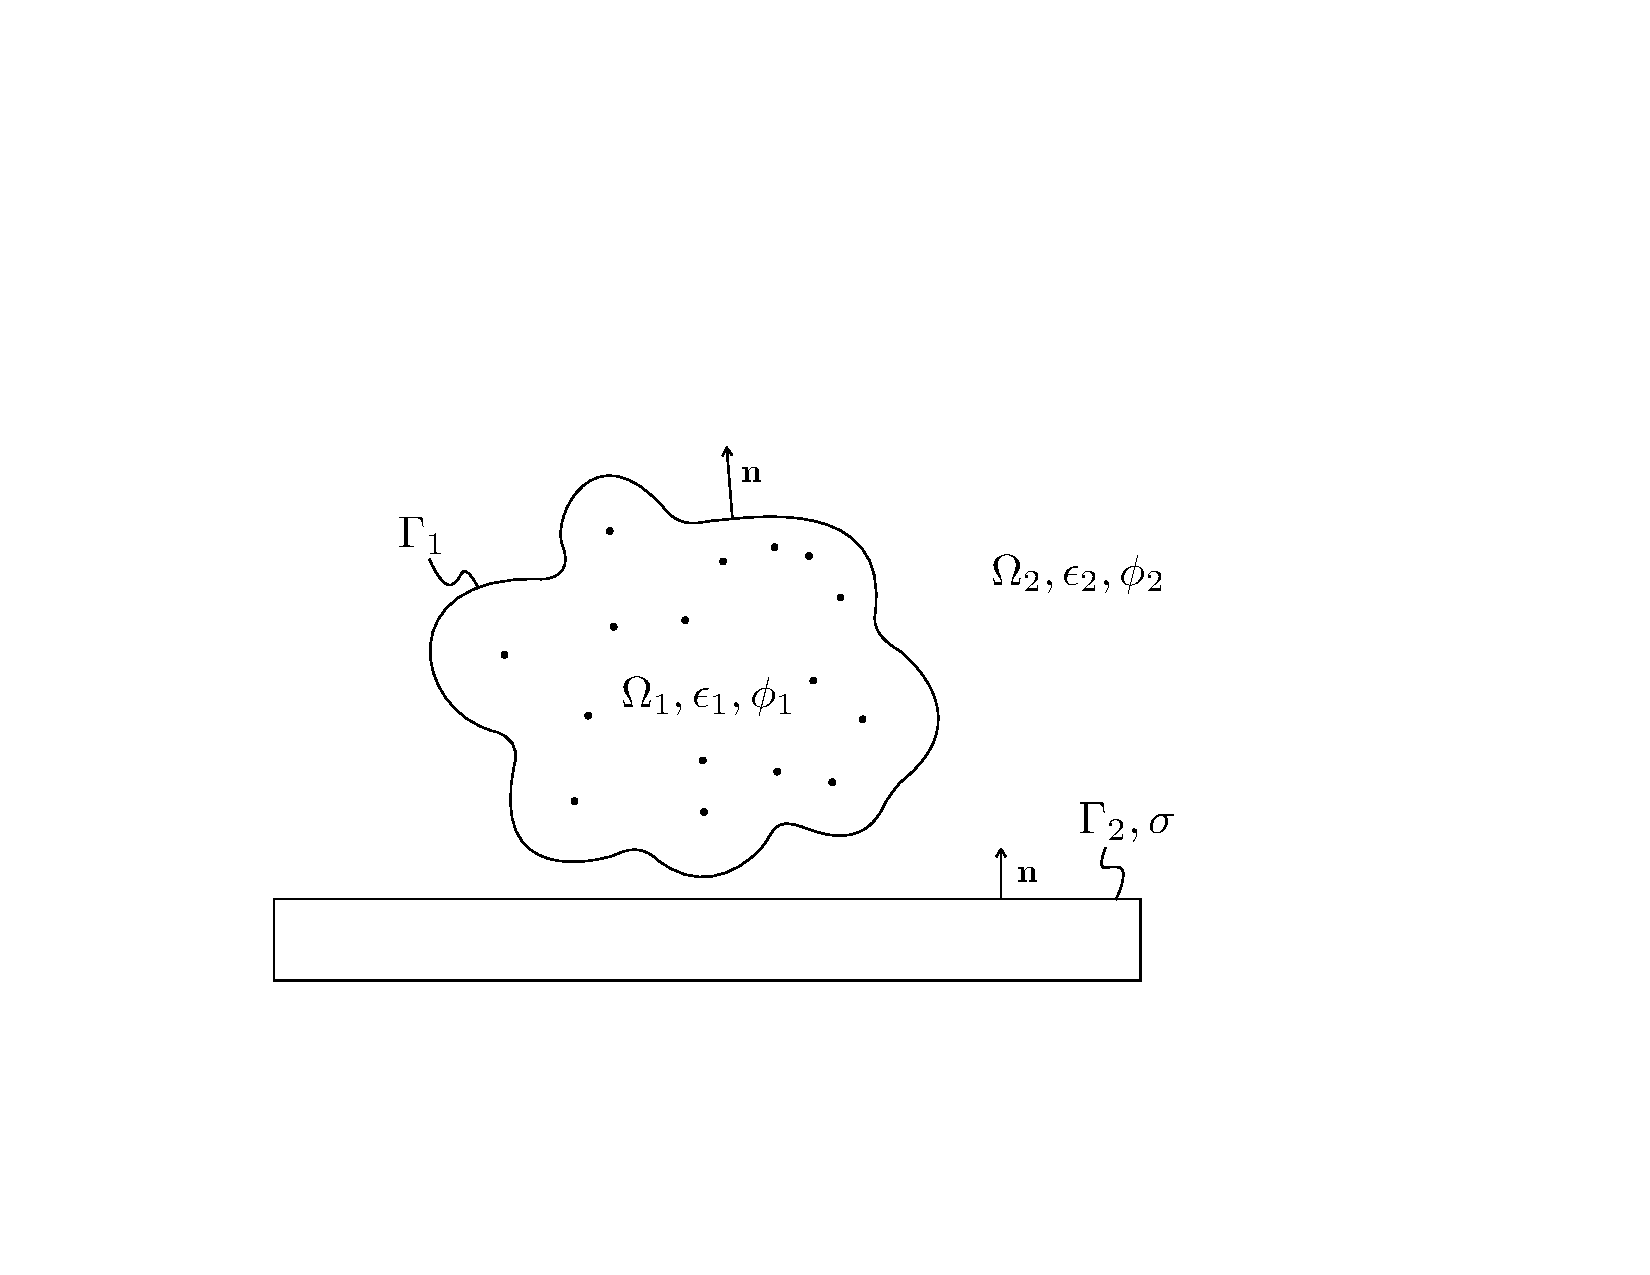
\includegraphics[width=0.45\textwidth]{Figure2.pdf} 
   \caption{Sketch of a molecule interacting with a surface: $\Omega_1$ is the protein, $\Omega_2$ the solvent region, $\Gamma_1$ is the  \ses and $\Gamma_2$ a nanosurface with imposed charge.}
   \label{fig:molecule_surface}
\end{figure}
